\documentclass[11]{article}

\usepackage[inline]{enumitem}
\usepackage{graphicx}
\usepackage{gensymb}
\usepackage{float}

\usepackage[numbered,framed]{matlab-prettifier}
\let\ph\mlplaceholder % shorter macro
\lstMakeShortInline"

\lstset{
  style              = Matlab-editor,
  basicstyle         = \mlttfamily,
  escapechar         = ",
  mlshowsectionrules = true,
}

\title{
  Hand Written
  Digit Recognition
  }
  
\date{}
\author{Adrian Ionita\\
\small{(NR: 1057404, ID: AFI904)}}

\hyphenation{thatshouldnot}

\begin{document}
\maketitle 	

\section{Introduction}
This project attempts to design a neural network to optically recognise hand written digits. Starting with the fewest number of layers and increasing subsequently, the network generalisation is optimised through adjusting parameters of learning rate, batch size, epoch count and data preprocessing. Weight decay was also used to further improve generalisation to a maximum performance of 97.21\% .

The data set used contains records from 43 participants and is split between a training set and a test set. The training set of 3823 records was collected from 30 of the participants. The test set of 1797 records was collected from the remaining 13. Each record contains 64 pixels of an 8x8 image (e.g. \ref{fig:digits} followed by the digit it represents. The pixel intensity is between 0 and 16. 

\begin{figure}[h]
\centering
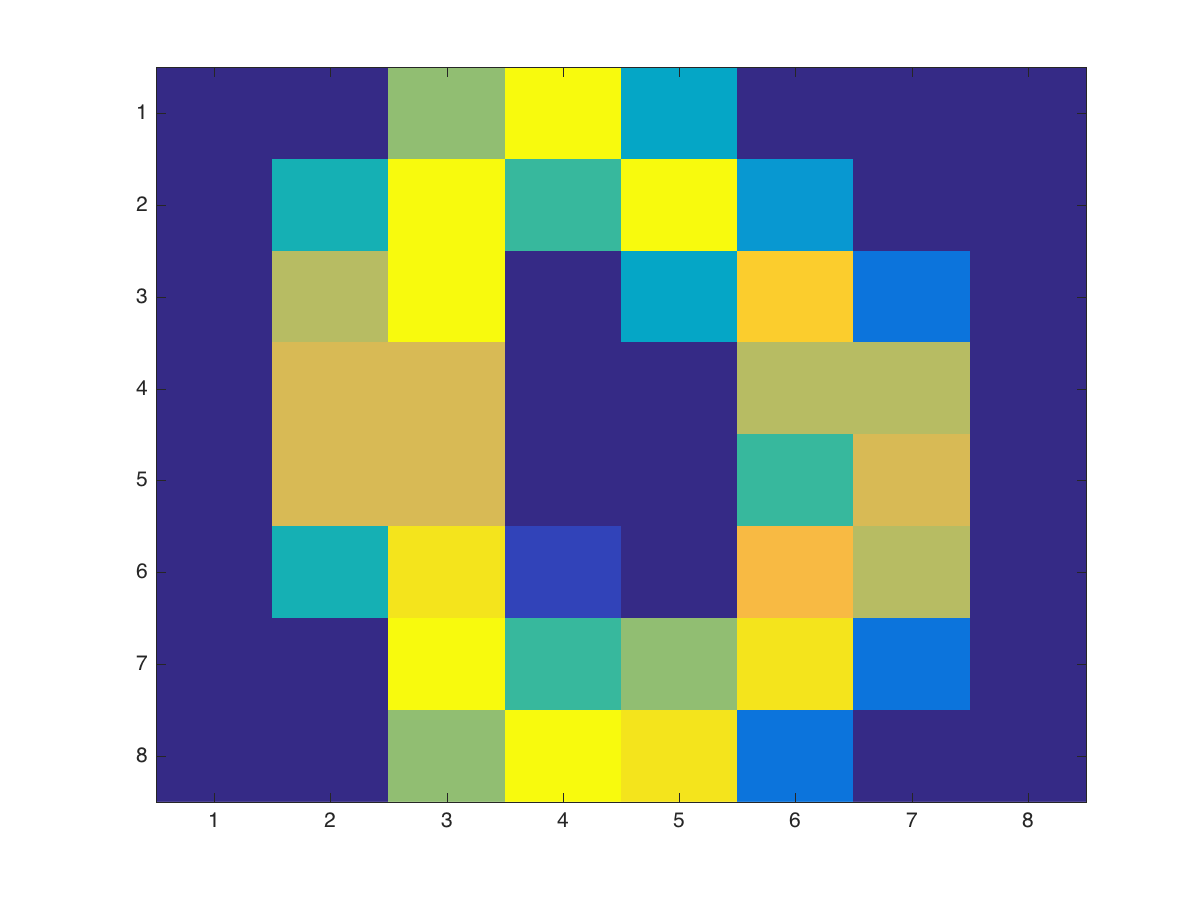
\includegraphics[width=0.4\textwidth]{zero.png}
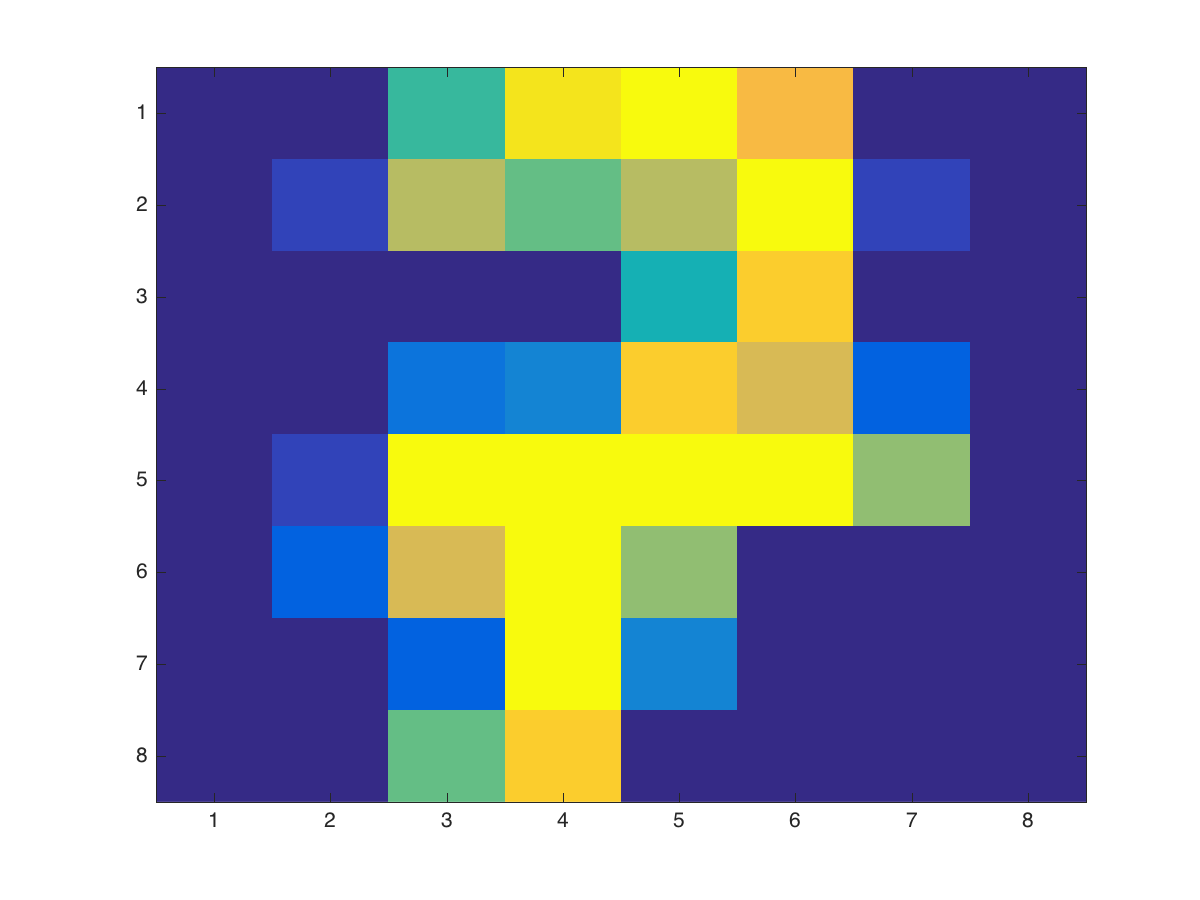
\includegraphics[width=0.4\textwidth]{seven.png}
\caption{Example images from training set}
\label{fig:digits}
\end{figure}
\section{Design}

The resulting design is a two layer perceptron neural network using the cross entropy cost function. This cost function was selected as the problem is one of classification rather than regression (i.e. each feature set belongs to a digit class).

When using cross entropy, the activation function generally used is a sigmoid. As its output ranges from 0 to 1, the activation of a neuron is analogous to a probability function. Whilst sigmoid is used for hidden layer activations, softmax is used for the output layer. This ensures that the probability of each class activation does not exceed 1. 

The network's input is 69 features. The fist 64 represent the image pixels with an additional 5 features extracted from pixel covariance and mean location.  The hidden layer size is 60 nodes and the output layer is 10 nodes ( one for each activation class ). 

Additional training sets were created by rotating each training set to a varying range between -20 and +20 degrees clockwise (fig. \ref{fig:rotated}. This is in order to aid detection of digits that are not properly aligned. The additional covariance and mean features of each record served the same purpose. 
\begin{figure}[h]
\centering
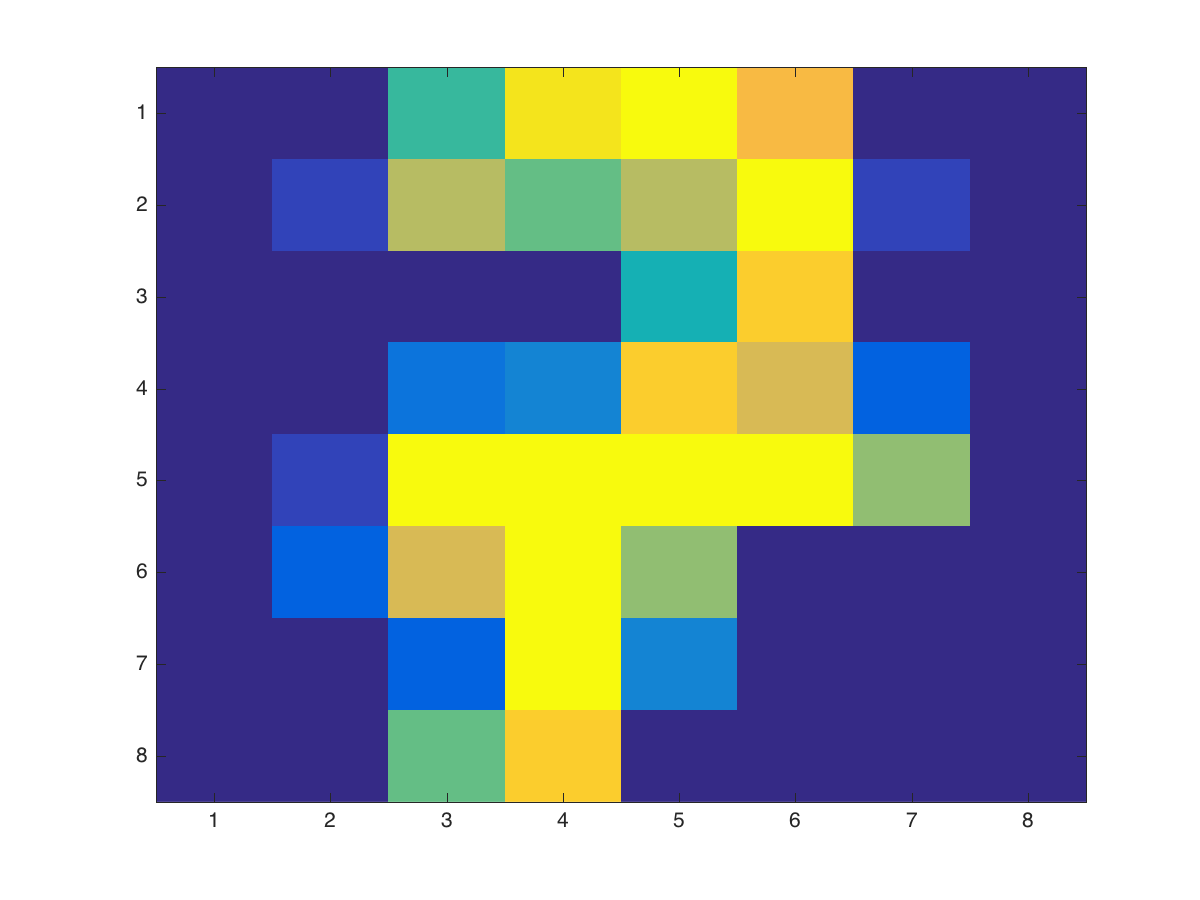
\includegraphics[width=0.4\textwidth]{seven.png}
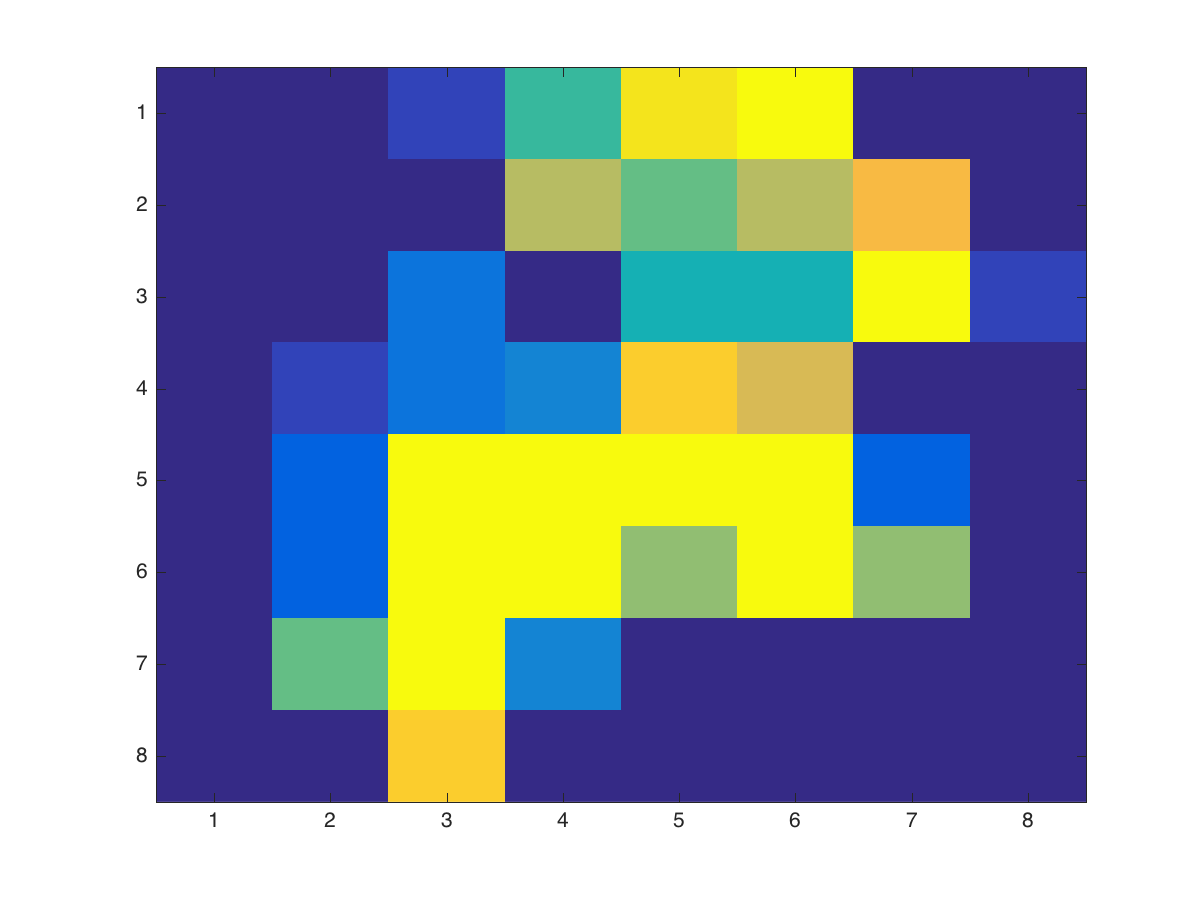
\includegraphics[width=0.4\textwidth]{seven_rotated.png}
\caption{Example images from training set}
\label{fig:rotated}
\end{figure}
\section{Design}

The network is trained off-line with a fixed batched size that was optimised experimentally. Batch training ensures a more smooth decent of the gradient error cost. Additionally a varying learning rate is used. This decreases in value with each complete iteration of the training set. The decay of the learning rate was optimised experimentally. There is one single learning rate used for both the output layer and hidden layers.

Network training stops after a fixed number of epochs was trained. An epoch was considered as one single update of the weights. Although the network may stop at a point where the error cost is high, the approach avoid situations where the network would never complete training ( i.e. when choosing an error cost that can't be achieved ). The optimal number of epochs was also discovered experimentally. 

Network training also employs a simple weight decay function ( i.e. decreasing the weights by a ratio of their current value. The decay ratio was optimised experimentally. 

\section{Implementation}

The neural network was implemented using matlab. Even though matlab has a specialised toolbox for neural networks, the project implements its own network and back-propagation algorithm. Matlab was chosen do to its in built matrix operations, mathematical tools and visualisation features (e.g. error cost plotting). When adding image rotations to the training set, the image processing toolbox further simplified code complexity as algorithms were readily available.

\subsection{Initialisation}

The entry file for training the network is \emph{train.m}. At the start of execution the training set is loaded and extended with additional records for digit rotations (using \emph{addrotations.m}). The resulting training set is three times larger, having one clockwise and one counter clockwise rotation for each digit. The set is then further extended with additional features (i.e. covariance and mean pixel location). After extension, the features are normalised and scaled up ( i.e. by multiplying each feature to a larger number). The feature extension and normalisation form a single step named preprocessing (handled by \emph{preprocess.m}).

The target class for the training set is separated from the rest of the features. Each target is transformed from a single digit to a 10 dimension vector. The vector represents the probability of each class occurring, meaning it has the value 1 on the class's position and 0 otherwise. 

\subsection{Training}

When training a network, it is first initialised with random weights drawn from a uniform distribution of $[-0.5,+0.5]$. The training is implented using vector and matrix multiplication instead of iterating through individual positions of weight updates. This takes advantage of matlab's optimisations in matrix operations and serves for faster training. 

The output of the hidden layer is first calculated using the sigmoid activation function on an input batch. It then gets used as input in calculating the total network output using the softmax function. These are handled, in vector notation, by \emph{sigmoid.m} and \emph{softmax.m}.
\begin{lstlisting}
        out{1} = sigmoid(in_batch,w{1});
        out{2} = softmax(out{1},w{2});
\end{lstlisting}

The delta of each weight update is calculated using the first derivative of the cost function for each layer (following course formulas). The weight are updated by the delta and also suffer a weight decay proportional to their current value. 

\subsection{Testing}

After training, the network weights are measured on the loaded test set. The set is processed similarly to the training one(i.e. through additional features and normalisation). When calculating the result of a given input, the predicted class is determined by selecting the output position with the highest probability value. Network performance is determined from the number of correctly predicted classes. 

\section{Experiments}

\subsection{Single Layer Experiments}
In order to establish a baseline of performance the network was initially built as a single layer perceptraon network with a fixed learning rate($\mu$), number of epochs and batch size. Each experiment trained and measured network performance 10 times for a better estimation of optimisation improvements. 

\subsubsection{Learning Rate}

For the initial training no preprocessing was done on the data set. Because of the softmax activation function, a batch size larger than 20 or a learning rate larger than 0.01 could not be used as the the function would overflow double precision data types.

With the initial batch=20, epoch=2000 and $\mu=0.01$, the network achieved 93.25\%($\pm 1.4\%)$ prediction success on the testing set.  A lower learning rate of $\mu=0.001$ was tried which produced a performance of 92.59\%($\pm 0.3\%$). Although the average performance was lower the deviation in learning was greatly reduced. Using a variable learning rate the performance was further improved to 94.57\%($\pm 0.07\%$) signifying a great improvement in both performance and stability (fig. \ref{fig:learningrate}). The learning rate decay per each complete iteration of the training set is defined as $\mu = \mu / 1.1$ starting with $\mu=0.01$. Reducing the rate by larger or lower ratio would not result in lower performance.
\begin{figure}[h]
\centering
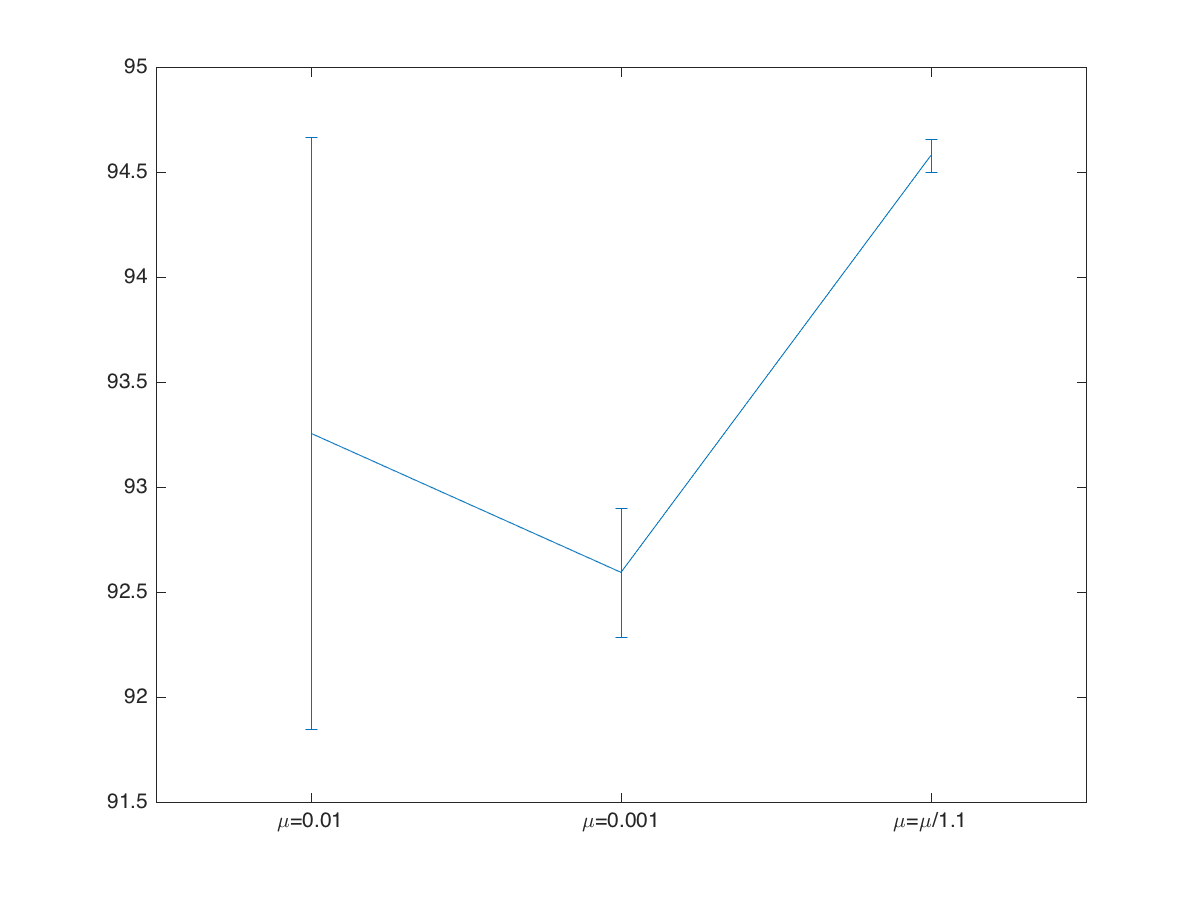
\includegraphics[width=0.6\textwidth]{learning_rate.png}
\caption{adjusting learning rate $\mu$}
\label{fig:learningrate}
\end{figure}

\subsubsection{Batch and Epoch Sizes}
Whilst a varying learning rate increase performance significantly, batch and epoch sizes were also experimented with (fig. \ref{fig:batchandepoch}). A low epoch size would underfit general training performance, whilst a low batch size would lead to larger deviations (as the gradient direction would be less stable). No performance improvements were achieved at this point. 

\begin{figure}[h]
\centering
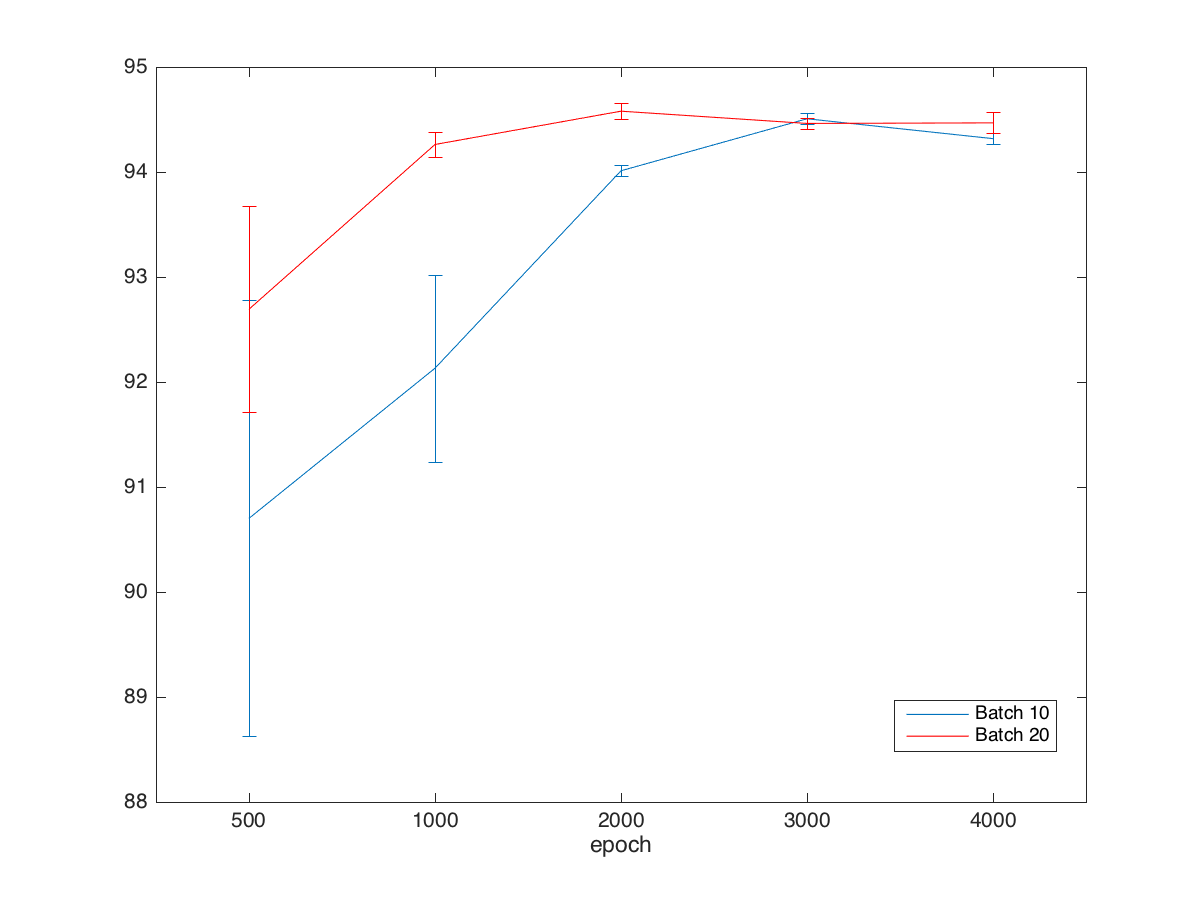
\includegraphics[width=0.6\textwidth]{batchandepoch.png}
\caption{adjusting the batch and epoch sizes}
\label{fig:batchandepoch}
\end{figure}

\subsubsection{Preprocessing}
To further increase performance, preprocessing was done to both the training and test sets. As mentioned previously, additional features were added. Feature values were normalised between $[0,12]$. Different scale intervals were tested although their results are not presented. 

The tenique improved average network performance to a mean of 95.11\%($\pm 0.01\%$) (fig. \ref{fig:normalised}). By normalising the data, the network could be trained with larger batch sizes and learning rates without number overflows. However, increasing these values did not further improve performance. 

\begin{figure}[h]
\centering
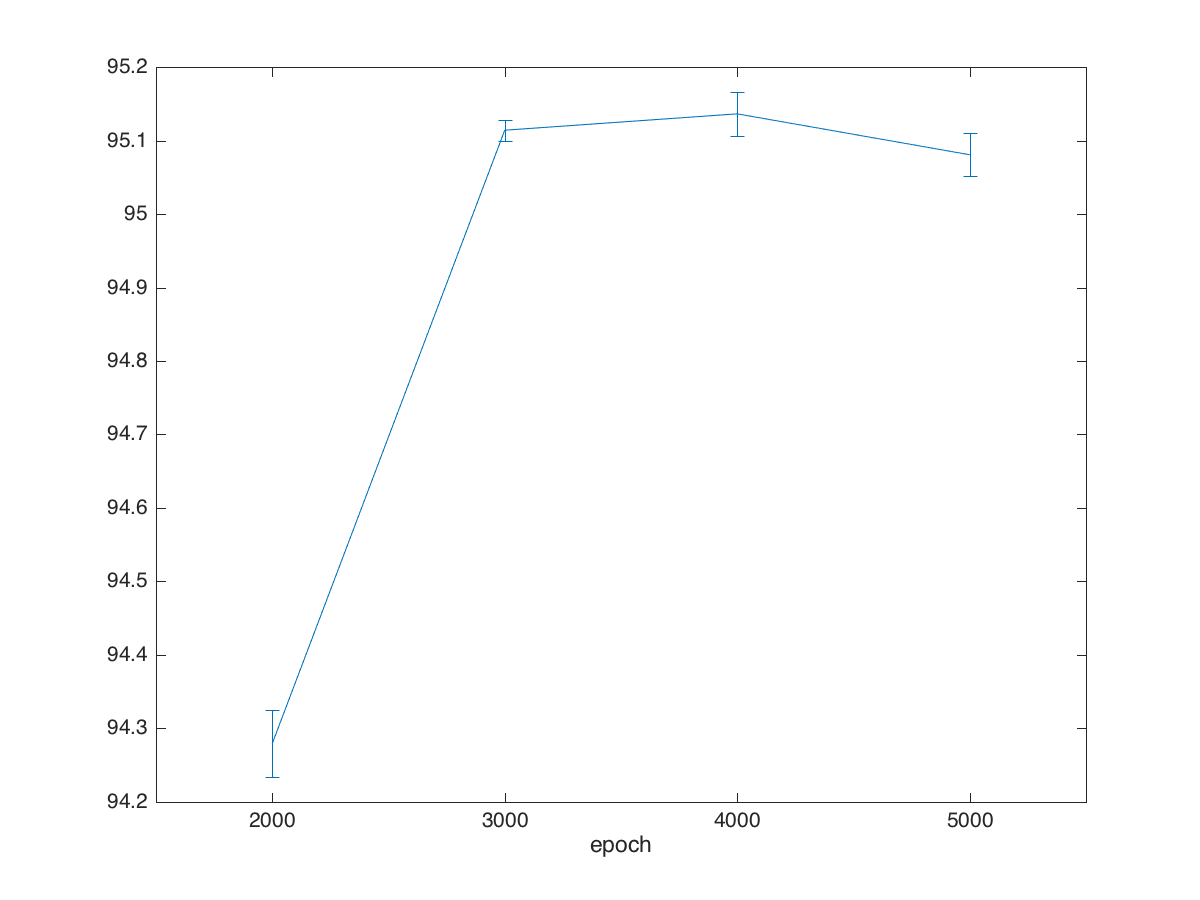
\includegraphics[width=0.6\textwidth]{normalised.png}
\caption{effects of adjusting the learning rate}
\label{fig:normalised}
\end{figure}

\subsection{Two Layer Experiments}

\section{Conclusions}

\begin{thebibliography}{9}
\bibitem{ucidigits}
UCI machine learning repository: Optical recognition of handwritten digits data set. (1998, July 1). Retrieved January 10, 2016, from http://archive.ics.uci.edu/ml/datasets/Optical+Recognition+of+Handwritten+Digits

\end{thebibliography}

\end{document}